
%% bare_conf.tex
%% V1.4b
%% 2015/08/26
%% by Michael Shell
%% See:
%% http://www.michaelshell.org/
%% for current contact information.
%%
%% This is a skeleton file demonstrating the use of IEEEtran.cls
%% (requires IEEEtran.cls version 1.8b or later) with an IEEE
%% conference paper.
%%
%% Support sites:
%% http://www.michaelshell.org/tex/ieeetran/
%% http://www.ctan.org/pkg/ieeetran
%% and
%% http://www.ieee.org/

%%*************************************************************************
%% Legal Notice:
%% This code is offered as-is without any warranty either expressed or
%% implied; without even the implied warranty of MERCHANTABILITY or
%% FITNESS FOR A PARTICULAR PURPOSE! 
%% User assumes all risk.
%% In no event shall the IEEE or any contributor to this code be liable for
%% any damages or losses, including, but not limited to, incidental,
%% consequential, or any other damages, resulting from the use or misuse
%% of any information contained here.
%%
%% All comments are the opinions of their respective authors and are not
%% necessarily endorsed by the IEEE.
%%
%% This work is distributed under the LaTeX Project Public License (LPPL)
%% ( http://www.latex-project.org/ ) version 1.3, and may be freely used,
%% distributed and modified. A copy of the LPPL, version 1.3, is included
%% in the base LaTeX documentation of all distributions of LaTeX released
%% 2003/12/01 or later.
%% Retain all contribution notices and credits.
%% ** Modified files should be clearly indicated as such, including  **
%% ** renaming them and changing author support contact information. **
%%*************************************************************************


% *** Authors should verify (and, if needed, correct) their LaTeX system  ***
% *** with the testflow diagnostic prior to trusting their LaTeX platform ***
% *** with production work. The IEEE's font choices and paper sizes can   ***
% *** trigger bugs that do not appear when using other class files.       ***                          ***
% The testflow support page is at:
% http://www.michaelshell.org/tex/testflow/



\documentclass[conference]{IEEEtran}
% Some Computer Society conferences also require the compsoc mode option,
% but others use the standard conference format.
%
% If IEEEtran.cls has not been installed into the LaTeX system files,
% manually specify the path to it like:
% \documentclass[conference]{../sty/IEEEtran}


\usepackage{url}


% Some very useful LaTeX packages include:
% (uncomment the ones you want to load)


% *** MISC UTILITY PACKAGES ***
%
%\usepackage{ifpdf}
% Heiko Oberdiek's ifpdf.sty is very useful if you need conditional
% compilation based on whether the output is pdf or dvi.
% usage:
% \ifpdf
%   % pdf code
% \else
%   % dvi code
% \fi
% The latest version of ifpdf.sty can be obtained from:
% http://www.ctan.org/pkg/ifpdf
% Also, note that IEEEtran.cls V1.7 and later provides a builtin
% \ifCLASSINFOpdf conditional that works the same way.
% When switching from latex to pdflatex and vice-versa, the compiler may
% have to be run twice to clear warning/error messages.






% *** CITATION PACKAGES ***
%
%\usepackage{cite}
% cite.sty was written by Donald Arseneau
% V1.6 and later of IEEEtran pre-defines the format of the cite.sty package
% \cite{} output to follow that of the IEEE. Loading the cite package will
% result in citation numbers being automatically sorted and properly
% "compressed/ranged". e.g., [1], [9], [2], [7], [5], [6] without using
% cite.sty will become [1], [2], [5]--[7], [9] using cite.sty. cite.sty's
% \cite will automatically add leading space, if needed. Use cite.sty's
% noadjust option (cite.sty V3.8 and later) if you want to turn this off
% such as if a citation ever needs to be enclosed in parenthesis.
% cite.sty is already installed on most LaTeX systems. Be sure and use
% version 5.0 (2009-03-20) and later if using hyperref.sty.
% The latest version can be obtained at:
% http://www.ctan.org/pkg/cite
% The documentation is contained in the cite.sty file itself.






% *** GRAPHICS RELATED PACKAGES ***
%
\ifCLASSINFOpdf
   \usepackage[pdftex]{graphicx}
  % declare the path(s) where your graphic files are
  % \graphicspath{{../pdf/}{../jpeg/}}
  % and their extensions so you won't have to specify these with
  % every instance of \includegraphics
  % \DeclareGraphicsExtensions{.pdf,.jpeg,.png}
\else
  % or other class option (dvipsone, dvipdf, if not using dvips). graphicx
  % will default to the driver specified in the system graphics.cfg if no
  % driver is specified.
   \usepackage[dvips]{graphicx}
  % declare the path(s) where your graphic files are
  % \graphicspath{{../eps/}}
  % and their extensions so you won't have to specify these with
  % every instance of \includegraphics
  % \DeclareGraphicsExtensions{.eps}
\fi
% graphicx was written by David Carlisle and Sebastian Rahtz. It is
% required if you want graphics, photos, etc. graphicx.sty is already
% installed on most LaTeX systems. The latest version and documentation
% can be obtained at: 
% http://www.ctan.org/pkg/graphicx
% Another good source of documentation is "Using Imported Graphics in
% LaTeX2e" by Keith Reckdahl which can be found at:
% http://www.ctan.org/pkg/epslatex
%
% latex, and pdflatex in dvi mode, support graphics in encapsulated
% postscript (.eps) format. pdflatex in pdf mode supports graphics
% in .pdf, .jpeg, .png and .mps (metapost) formats. Users should ensure
% that all non-photo figures use a vector format (.eps, .pdf, .mps) and
% not a bitmapped formats (.jpeg, .png). The IEEE frowns on bitmapped formats
% which can result in "jaggedy"/blurry rendering of lines and letters as
% well as large increases in file sizes.
%
% You can find documentation about the pdfTeX application at:
% http://www.tug.org/applications/pdftex





% *** MATH PACKAGES ***
%
%\usepackage{amsmath}
% A popular package from the American Mathematical Society that provides
% many useful and powerful commands for dealing with mathematics.
%
% Note that the amsmath package sets \interdisplaylinepenalty to 10000
% thus preventing page breaks from occurring within multiline equations. Use:
%\interdisplaylinepenalty=2500
% after loading amsmath to restore such page breaks as IEEEtran.cls normally
% does. amsmath.sty is already installed on most LaTeX systems. The latest
% version and documentation can be obtained at:
% http://www.ctan.org/pkg/amsmath





% *** SPECIALIZED LIST PACKAGES ***
%
%\usepackage{algorithmic}
% algorithmic.sty was written by Peter Williams and Rogerio Brito.
% This package provides an algorithmic environment fo describing algorithms.
% You can use the algorithmic environment in-text or within a figure
% environment to provide for a floating algorithm. Do NOT use the algorithm
% floating environment provided by algorithm.sty (by the same authors) or
% algorithm2e.sty (by Christophe Fiorio) as the IEEE does not use dedicated
% algorithm float types and packages that provide these will not provide
% correct IEEE style captions. The latest version and documentation of
% algorithmic.sty can be obtained at:
% http://www.ctan.org/pkg/algorithms
% Also of interest may be the (relatively newer and more customizable)
% algorithmicx.sty package by Szasz Janos:
% http://www.ctan.org/pkg/algorithmicx




% *** ALIGNMENT PACKAGES ***
%
%\usepackage{array}
% Frank Mittelbach's and David Carlisle's array.sty patches and improves
% the standard LaTeX2e array and tabular environments to provide better
% appearance and additional user controls. As the default LaTeX2e table
% generation code is lacking to the point of almost being broken with
% respect to the quality of the end results, all users are strongly
% advised to use an enhanced (at the very least that provided by array.sty)
% set of table tools. array.sty is already installed on most systems. The
% latest version and documentation can be obtained at:
% http://www.ctan.org/pkg/array


% IEEEtran contains the IEEEeqnarray family of commands that can be used to
% generate multiline equations as well as matrices, tables, etc., of high
% quality.




% *** SUBFIGURE PACKAGES ***
%\ifCLASSOPTIONcompsoc
%  \usepackage[caption=false,font=normalsize,labelfont=sf,textfont=sf]{subfig}
%\else
%  \usepackage[caption=false,font=footnotesize]{subfig}
%\fi
% subfig.sty, written by Steven Douglas Cochran, is the modern replacement
% for subfigure.sty, the latter of which is no longer maintained and is
% incompatible with some LaTeX packages including fixltx2e. However,
% subfig.sty requires and automatically loads Axel Sommerfeldt's caption.sty
% which will override IEEEtran.cls' handling of captions and this will result
% in non-IEEE style figure/table captions. To prevent this problem, be sure
% and invoke subfig.sty's "caption=false" package option (available since
% subfig.sty version 1.3, 2005/06/28) as this is will preserve IEEEtran.cls
% handling of captions.
% Note that the Computer Society format requires a larger sans serif font
% than the serif footnote size font used in traditional IEEE formatting
% and thus the need to invoke different subfig.sty package options depending
% on whether compsoc mode has been enabled.
%
% The latest version and documentation of subfig.sty can be obtained at:
% http://www.ctan.org/pkg/subfig




% *** FLOAT PACKAGES ***
%
%\usepackage{fixltx2e}
% fixltx2e, the successor to the earlier fix2col.sty, was written by
% Frank Mittelbach and David Carlisle. This package corrects a few problems
% in the LaTeX2e kernel, the most notable of which is that in current
% LaTeX2e releases, the ordering of single and double column floats is not
% guaranteed to be preserved. Thus, an unpatched LaTeX2e can allow a
% single column figure to be placed prior to an earlier double column
% figure.
% Be aware that LaTeX2e kernels dated 2015 and later have fixltx2e.sty's
% corrections already built into the system in which case a warning will
% be issued if an attempt is made to load fixltx2e.sty as it is no longer
% needed.
% The latest version and documentation can be found at:
% http://www.ctan.org/pkg/fixltx2e


%\usepackage{stfloats}
% stfloats.sty was written by Sigitas Tolusis. This package gives LaTeX2e
% the ability to do double column floats at the bottom of the page as well
% as the top. (e.g., "\begin{figure*}[!b]" is not normally possible in
% LaTeX2e). It also provides a command:
%\fnbelowfloat
% to enable the placement of footnotes below bottom floats (the standard
% LaTeX2e kernel puts them above bottom floats). This is an invasive package
% which rewrites many portions of the LaTeX2e float routines. It may not work
% with other packages that modify the LaTeX2e float routines. The latest
% version and documentation can be obtained at:
% http://www.ctan.org/pkg/stfloats
% Do not use the stfloats baselinefloat ability as the IEEE does not allow
% \baselineskip to stretch. Authors submitting work to the IEEE should note
% that the IEEE rarely uses double column equations and that authors should try
% to avoid such use. Do not be tempted to use the cuted.sty or midfloat.sty
% packages (also by Sigitas Tolusis) as the IEEE does not format its papers in
% such ways.
% Do not attempt to use stfloats with fixltx2e as they are incompatible.
% Instead, use Morten Hogholm'a dblfloatfix which combines the features
% of both fixltx2e and stfloats:
%
% \usepackage{dblfloatfix}
% The latest version can be found at:
% http://www.ctan.org/pkg/dblfloatfix




% *** PDF, URL AND HYPERLINK PACKAGES ***
%
%\usepackage{url}
% url.sty was written by Donald Arseneau. It provides better support for
% handling and breaking URLs. url.sty is already installed on most LaTeX
% systems. The latest version and documentation can be obtained at:
% http://www.ctan.org/pkg/url
% Basically, \url{my_url_here}.




% *** Do not adjust lengths that control margins, column widths, etc. ***
% *** Do not use packages that alter fonts (such as pslatex).         ***
% There should be no need to do such things with IEEEtran.cls V1.6 and later.
% (Unless specifically asked to do so by the journal or conference you plan
% to submit to, of course. )


% correct bad hyphenation here
\hyphenation{op-tical net-works semi-conduc-tor}


\begin{document}
%
% paper title
% Titles are generally capitalized except for words such as a, an, and, as,
% at, but, by, for, in, nor, of, on, or, the, to and up, which are usually
% not capitalized unless they are the first or last word of the title.
% Linebreaks \\ can be used within to get better formatting as desired.
% Do not put math or special symbols in the title.
\title{Deep Q-Learning for Autonomous Driving}


% author names and affiliations
% use a multiple column layout for up to three different
% affiliations

% conference papers do not typically use \thanks and this command
% is locked out in conference mode. If really needed, such as for
% the acknowledgment of grants, issue a \IEEEoverridecommandlockouts
% after \documentclass

% for over three affiliations, or if they all won't fit within the width
% of the page, use this alternative format:
% 
\author{\IEEEauthorblockN{
Andr\'{e} Bauer,
Fabian D\"urr,
Jonathan H\"artl, 
Xiaoli Ma and
Kun Nie}
\IEEEauthorblockA{FZI\\
Karlsruhe Institute of Technology}}




% use for special paper notices
%\IEEEspecialpapernotice{(Invited Paper)}




% make the title area
\maketitle

% As a general rule, do not put math, special symbols or citations
% in the abstract
%!TEX root = bare_conf.tex

\begin{abstract}
	What we did
\end{abstract}

% no keywords




% For peer review papers, you can put extra information on the cover
% page as needed:
% \ifCLASSOPTIONpeerreview
% \begin{center} \bfseries EDICS Category: 3-BBND \end{center}
% \fi
%
% For peerreview papers, this IEEEtran command inserts a page break and
% creates the second title. It will be ignored for other modes.
\IEEEpeerreviewmaketitle


%!TEX root = bare_conf.tex

\section{Introduction}

In the last couple of years autonomous driving became a hot discussed topic. The approaches used for autonomous driving generally fall in one of two categories: mediated perception or behaviour reflex. The first one treats the whole system as a combination of multiple sub-systems. Each sub-system takes responsibility for one specific task, such as lane detection, traffic light detection, pedestrian detection and more. The features obtained from each sub-system are then fused together to form a single decision. Behaviour reflex approaches do not use mediated sub-systems, instead decisions are made directly based on the raw sensor data.

Deep learning has proven to be a powerful tool for image processing, especially convolutional neural networks (CNN), which are able to learn a high level abstraction of the input data by extracting features of different levels. Reinforcement learning is a powerful tool to address problems in decision making without knowing the underlying model. Deep-Q-learning (DQN) combines both of these two methods, by approximating the Q-function of a Q-learning approach with a deep neural network. First introduced in \cite{Mnih13} by Mnih et al., human level results for playing Atari games were achieved. Yu et al. \cite{yudeep} had success in the autonomous control of a vehicle in a Java Script based game using DQN and Chen et al. \cite{chen2015deepdriving} made advances in the complexity of the environment that could be learned. In this paper we present a behaviour reflex approach using DQN to teach an autonomous vehicle to drive in a 3D simulation. 

In Section \ref{sec:setup} we will introduce the fundamental architecture and setup of our system. The approach, including network, training and reward function, will be discussed in section \ref{sec:approach}. Next we will evaluate our approach in \ref{sec:evaluation}. Lastly, in \ref{sec:discussion} we will discuss our work and present an outlook for further development.

%!TEX root = bare_conf.tex

\begin{figure}[!t]
	\centering
	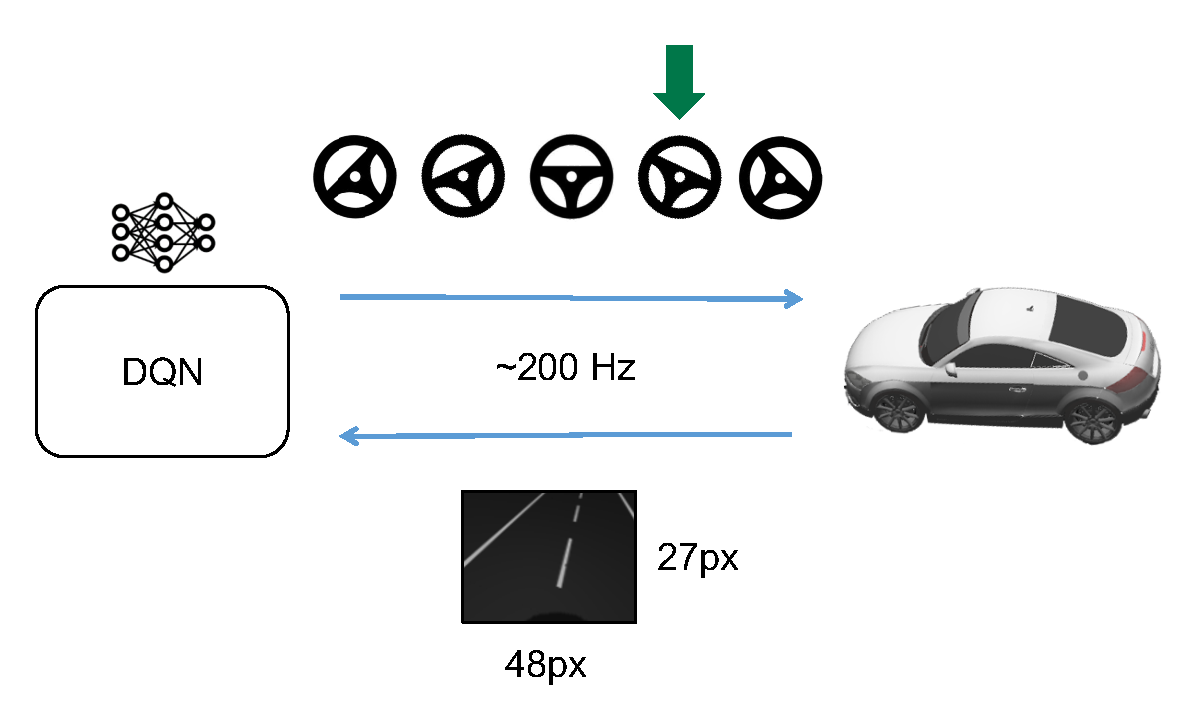
\includegraphics[width=3.5in]{../presentation/archi} 
	\caption{System architecture: Every time the simulation (depicted as vehicle) sends a camera image to DQN, a set of Q-values are calculated by the net, one for each action. The action corresponding to the largest Q-value is selected. As an example here the action: \textit{Half-right} is selected.}
	\label{fig:archi}
\end{figure}

\section{Setup} \label{sec:setup}
Gazebo\footnote{\url{http://gazebosim.org}} was used as the simulation environment. We had one car model and a small tileset of track pieces at our disposal to build custom tracks. The car was almost as wide as an entire lane, which made the task even more challenging. We were given plug-ins, which simplified the controls to setting a speed value in $[-1, 1]$ and a steering angle in $[-1, 1]$.

We selected Caffe\cite{jia2014caffe} as deep learning framework and Ros \footnote{\url{http://www.ros.org}} was chosen as a tool for the communication between DQN and Gazebo.

%!TEX root = bare_conf.tex

\section{Approach}\label{sec:approach}

In order to solve the task of autonomous driving in the simulation environment we had to make some fundamental decisions. First of all we specified our input source. The image of a front facing camera was chosen as input, because it provides more than enough information for this task. Secondly we decided to use an action set of five actions. The angles of \textit{Left} and \textit{Right} were chosen that the car complete even the tightest curves. The actions and their values are listed below. To support the mentioned input and generate the required output the given network was altered as described in the following section.
\begin{center}
	\begin{tabular}{ l | r | l }
							&	angle	& speed\\
		\hline
		\textit{Left} 		& 	-0.4 	& 0.6	\\
		\textit{Half-left} 	& 	-0.2 	& 0.6	\\
		\textit{Straight} 	& 	0 		& 0.6	\\
		\textit{Half-right} & 	0.2 	& 0.6	\\
		\textit{Right} 		& 	0.4 	& 0.6	\\
	\end{tabular}\\
	see \ref{sec:setup} for explanation of values
	\label{actionset}
\end{center}

\subsection{Network}
The network we use is based on the one introduced by Mnih et al. \cite{Mnih13}. Instead of four frames we process only one frame at a time, because lane following at constant speed does not require temporal context. The input image is reduced to 48 $\times$ 27 grayscale. At this resolution the camera image still contains enough information on the lane markings. The network has two convolution layers and two fully connected layers. Both convolutional layers use 4 $\times$ 4 kernels with a stride of 2. Layer one learns 16 filters, while layer two learns 32. The first fully connected layer has 256 neurons. The second fully connected layer computes 5 outputs, which represent the Q value for each action.

%-Structure + Parameters
%-Input
%-Output / Actions

\subsection{Training}
The framework used for training is an implementation of the paper ''Playing Atari with Deep Reinforcement Learning``  created by Peter Wolf. We altered some training parameters to adapt the framework to our needs. Therefore we set the size of the replay memory to 500k, in order to use the maximum memory available on the machine which was 16GB. The exploration value varied from 2 million Iterations up to 5 million, depending on the estimated training complexity. We also limit the length of an episode to 10k actions, to ensure a valid position of the car. An episode may end before reaching this limit, if the car leaves the driving lane. At the beginning of each episode the car is randomly placed on the track. This is done to ensure the entire track gets explored early on.

In training the weights of the network are adjusted every iteration. By default the simulation continues while updating the weights. To avoid frame skips in training that are not present while evaluating, we decided to pause the simulation while updating the weights.

For the network an initial learning rate of $10^{-5}$ is chosen, which is decreased by a factor of 0.1 every 2 million iterations.

These settings allowed us to complete 3 to 4 million training iterations per day. The plots in figure \ref{fig:lossandrew} show that the training is finished after 6 million iterations. That means that approximately 48 hours of training are needed every time a change is made.

\begin{figure}[!t]
\centering
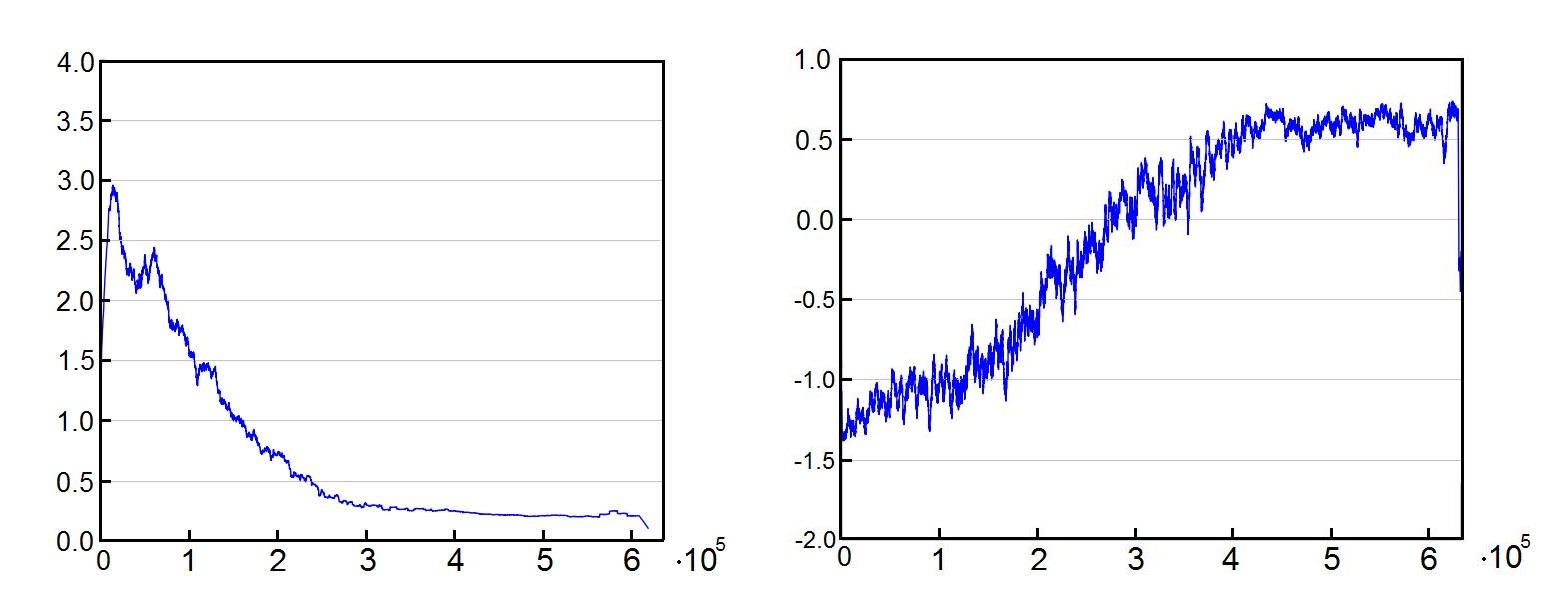
\includegraphics[width=3.5in]{../presentation/both-plot.jpg} 
\caption{Left: Loss of the network for one training. Right: Reward collected by the car. After approximately 4 million iterations both values are converged.}
\label{fig:lossandrew}
\end{figure}
 
%-Trainings params
%-Performance 
%-Pause physics
%-Loss + Reward plots

\begin{figure}[!t]
\centering
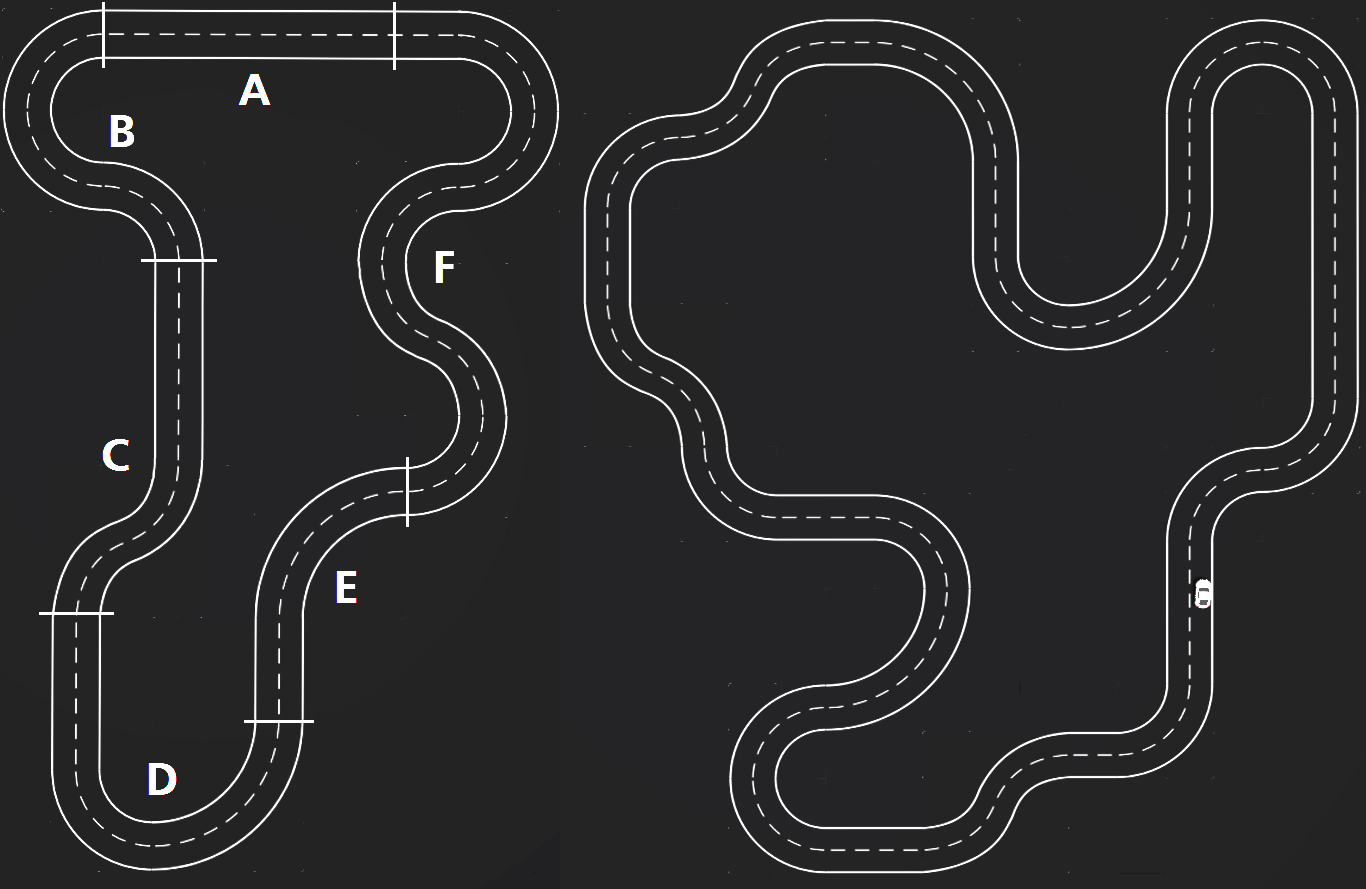
\includegraphics[scale=0.24]{../plots/track_both}
\caption{Left: Training track divided in six sections. Right: Additional test track with vehicle.}
\label{track}
\end{figure}

\begin{figure*}[!t]
\centering
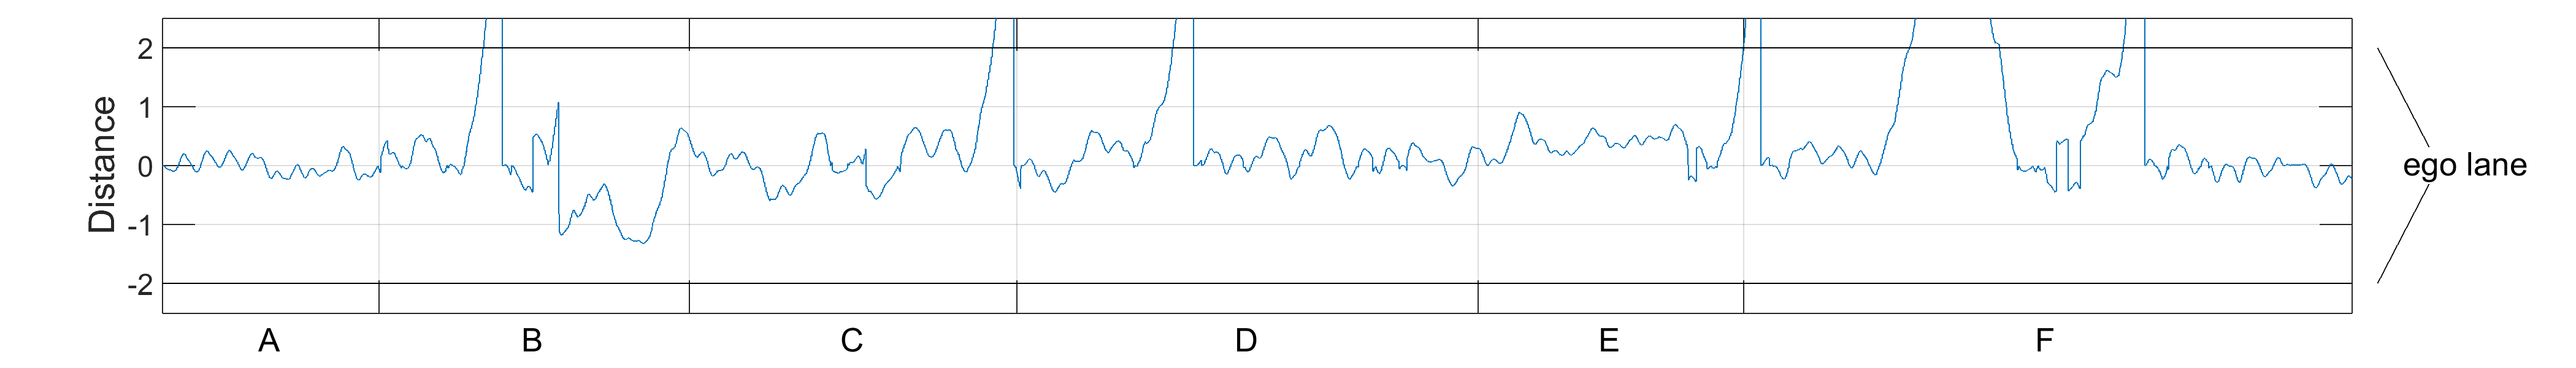
\includegraphics[scale=0.265]{../plots/dist_eval_log_distance_serpentine_06speed}
\vspace{0.5em}
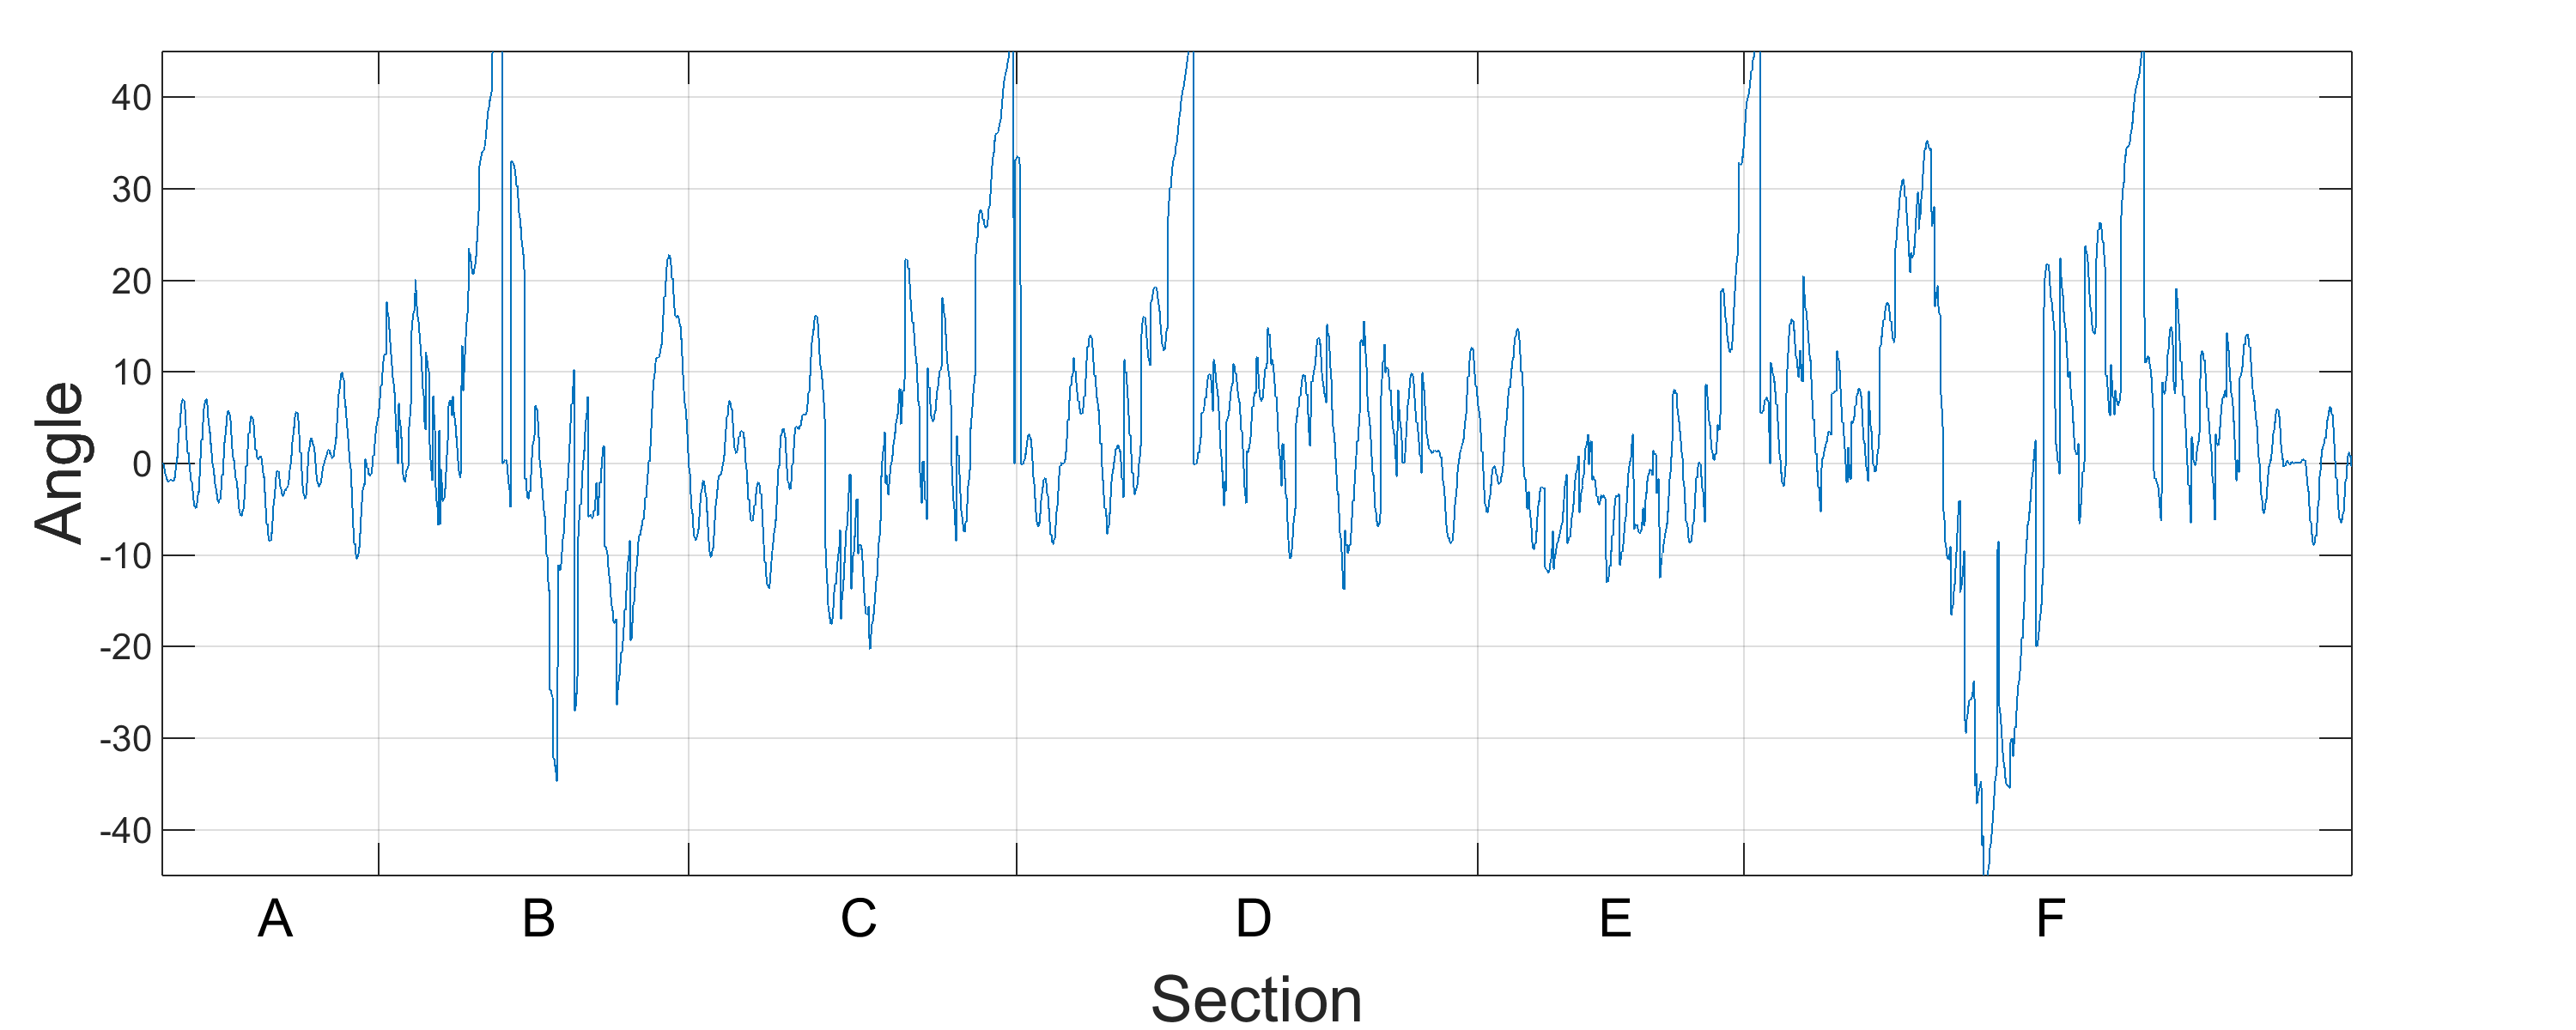
\includegraphics[scale=0.265]{../plots/ang_eval_log_distance_serpentine_06speed}
\vspace{-2.25em}
\caption{Distance-only approach. Distance in meters, angle in degrees.}
\label{distance06}
\vspace{1em}
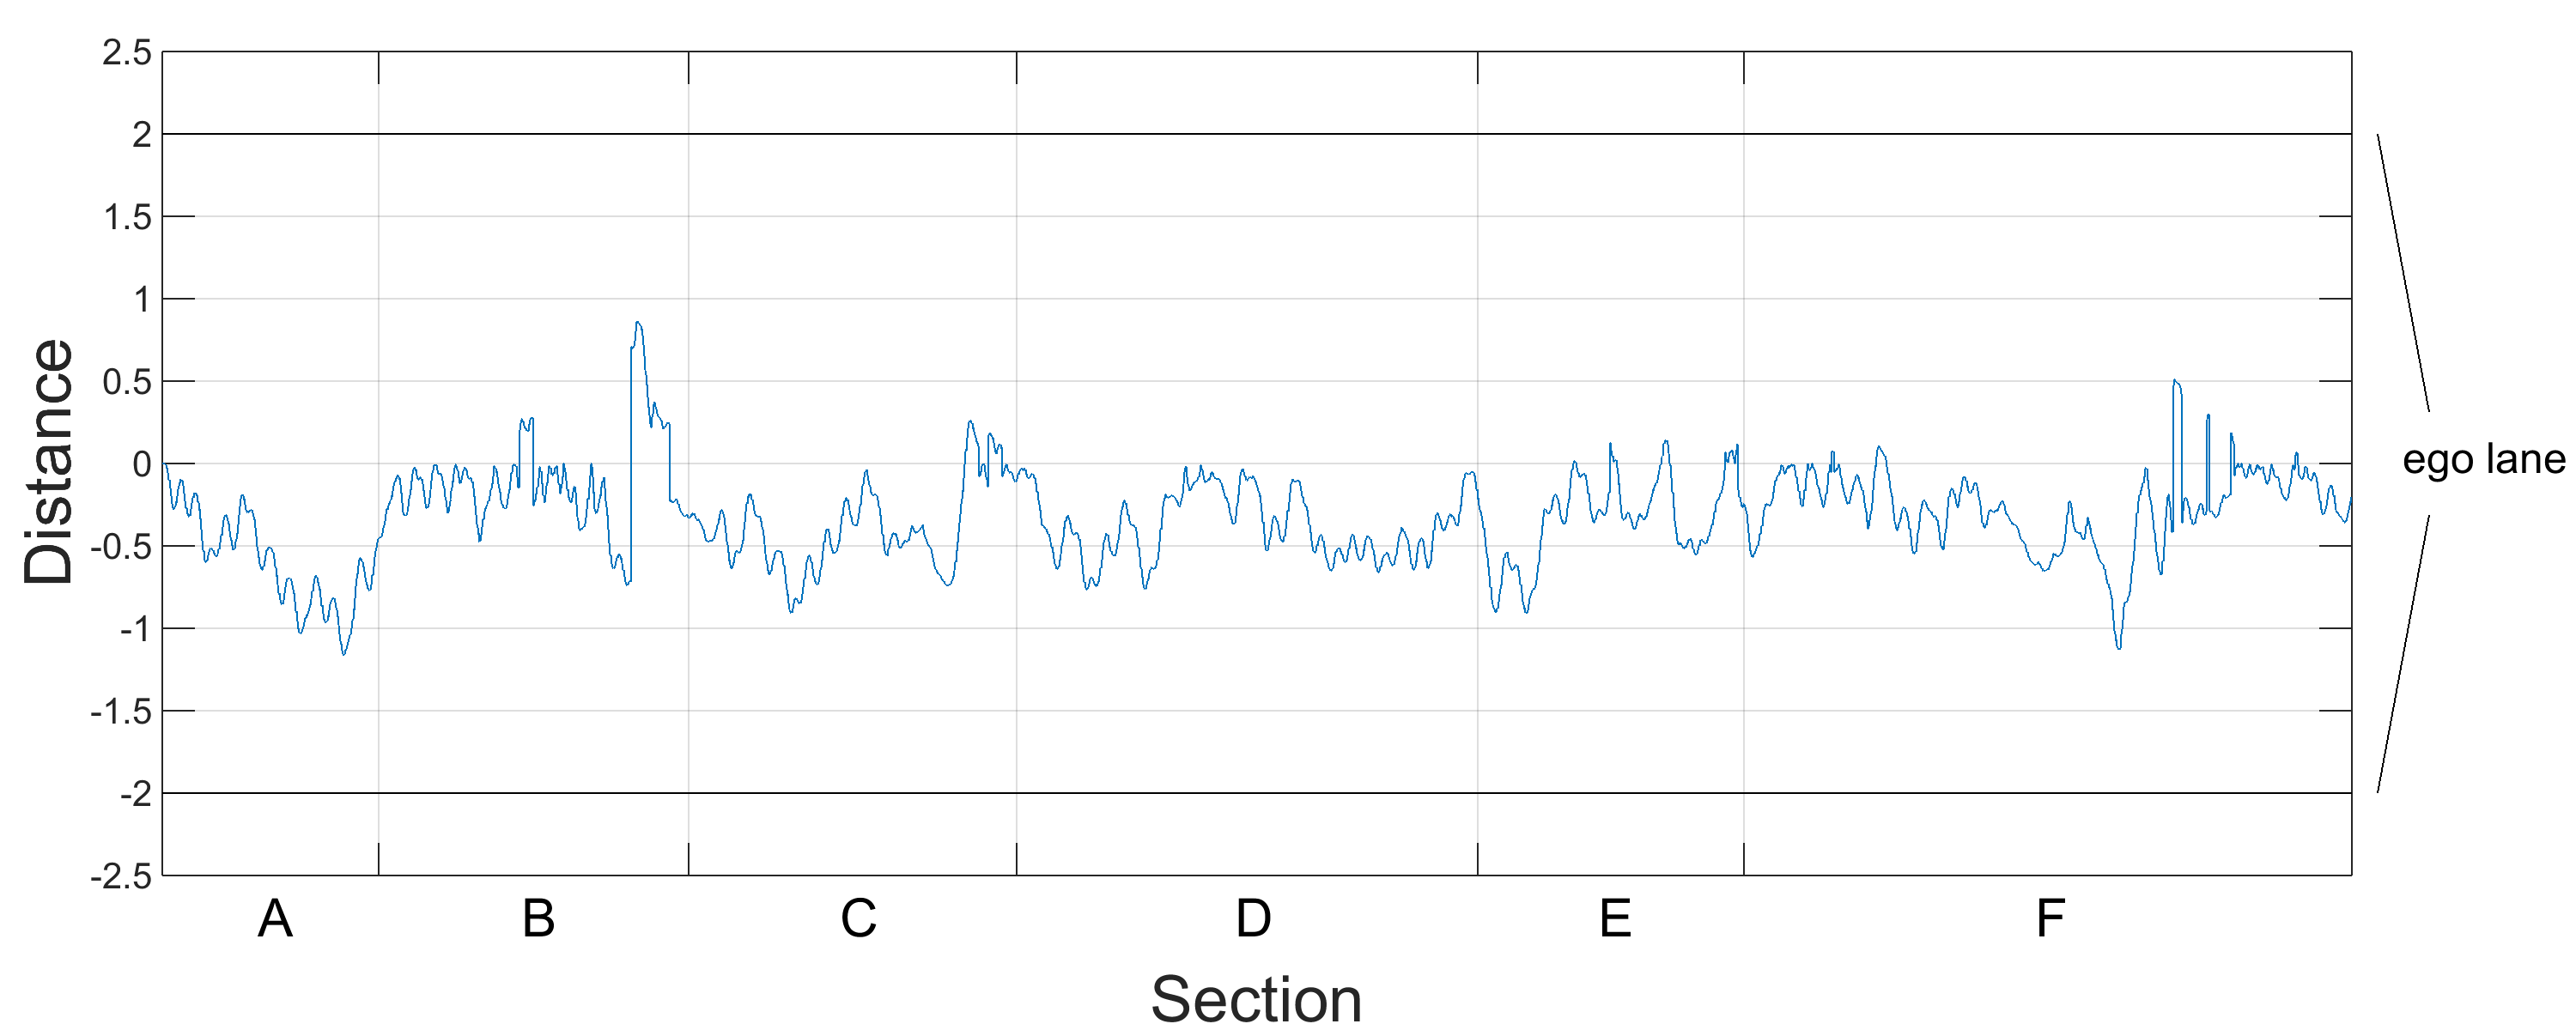
\includegraphics[scale=0.265]{../plots/dist_eval_log_dumb_actions_serpentine_06speed}
\vspace{0.5em}
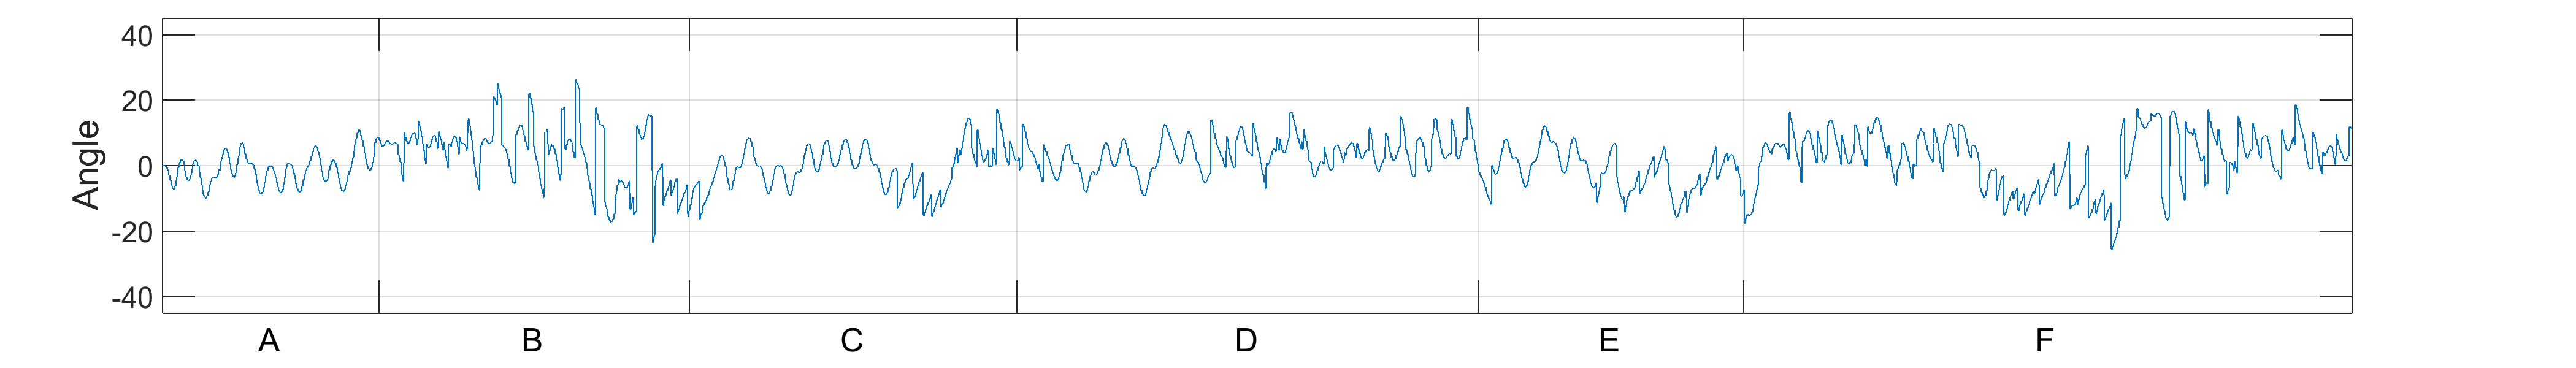
\includegraphics[scale=0.265]{../plots/ang_eval_log_dumb_actions_serpentine_06speed}
\vspace{-2.25em}
\caption{First action punishment added. Distance in meters, angle in degrees.}
\label{dumbactions06}
\end{figure*}

\subsection{Reward function}
The behaviour of the car is controlled through the reward function, hence any changes need to be done advisedly. As soon as the framework was up and running almost the entire development time was designated for testing of various functions. 

To ease development we decided to display a color coding of the current reward directly on the vehicle. This allowed us to check, before launching a new training, if the changes made to the reward function promised noteworthy gains or if they contained any errors. 
%-to ease development of reward function -> coloring
%-plot distance 
\subsubsection{Distance based}
A distance function serves as an intuitive starting point to teach the car where it is currently located in relation to the road. There are several problems with this simple approach though. The current distance is not a result of the currently chosen action, but the one of the past actions up to this point. While Q-learning methods do account for this, having a delayed reward does drag out the training time. Furthermore there is no feedback concerning the cars orientation in relation to the road. This can result in good rewards even though the car is arbitrarily oriented. As a consequence driving behaviour will be anything but smooth. The distance function we used was:
\[ r_D(d) = 2 - (|d| + 1)^6 \]
Where d is the distance in meters to the center of the lane. We wanted a maximum distance reward of +1 followed by a steep fall off to both sides of the lane.
\subsubsection{Distance and Action based}
To tackle the lack of immediate feedback we used several action assessments. Depending on the current state, some actions can only be decremental and should therefore be punished while others may be beneficial and should be rewarded. One important thing to note here is to handle the balance between distance and action based rewards with care. If one is weighted too heavily, the other one might get ignored, resulting in a performance decrease.

First we added a punishment if the car was on one side of the road, oriented away from it and also steering away from it. While this might be a useful action for advanced tasks, it is not at any time helpful to stay in the lane.

Next was optimizing the behaviour on a straight road. We give an additional reward if the car is located on a straight road, is in proximity to the center of the lane and chooses to steer straight.

Lastly we punished countersteering in curves. While human drivers often do exploit this to stay in lane, we hoped for a smoother result if the car made less use of it.

As they are separated by situation and action, only one of the above action reward rules can trigger at any given time. Considering the above rules we decide for a given state $x$ and action $a$ whether the usage of $a$ in $x$ is beneficial $(x, a) \in B$, or decremental $(x, a) \in D$.
\[ r_A(x, a) = 
	\begin{cases}
		+1	&	, (x, a) \in B\\
		-1	&	, (x, a) \in D\\		
		0	&	, else\\
	\end{cases}
\]
The reward function is obtained by simple addition. The distance reward was capped to keep the balance between $r_D$ and $r_A$ intact for larger distances. 
\[ r = \max(r_D\text{, }-2) + r_A \]

%!TEX root = bare_conf.tex

\section{Evaluation}
-RMSE plots for distance and angle?
-for different track



%!TEX root = bare_conf.tex

\section{Discussion}\label{sec:discussion}

%-obstacles
%-deltas
%-real world
From this project we can draw some conclusions. Firstly, selection of reward functions is very important. With a bad reward function the agent could learn nothing. Secondly, the training can also be successful even with a small net and small image. The deep neural networks we used is much smaller than the ones such as AlexNet or VGG. Finally, improper actions can lead to bad performance. For example, when we set the car a large speed, it can not follow the lanes any more.

However, it is difficult to transfer the success of this project to an application for real self-driving cars. In order to get more realistic results, some further experiments are needed be carried out. For instance, the car can be trained on more complex routes with traffic, crossing or obstacles. Furthermore, the steering angle in the actions must not remain fixed. They could have a ``delta'' increment. So the actions for turning could be ``more'' or ``less'' left and ``more'' or ``less'' right. We could take current steering angle along with the image as input of DQN. With this the car should run more smoothly at curves. 



% conference papers do not normally have an appendix


% use section* for acknowledgment
\section*{Acknowledgment}


The authors would like to thank...


% An example of a floating figure using the graphicx package.
% Note that \label must occur AFTER (or within) \caption.
% For figures, \caption should occur after the \includegraphics.
% Note that IEEEtran v1.7 and later has special internal code that
% is designed to preserve the operation of \label within \caption
% even when the captionsoff option is in effect. However, because
% of issues like this, it may be the safest practice to put all your
% \label just after \caption rather than within \caption{}.
%
% Reminder: the "draftcls" or "draftclsnofoot", not "draft", class
% option should be used if it is desired that the figures are to be
% displayed while in draft mode.
%
%\begin{figure}[!t]
%\centering
%\includegraphics[width=2.5in]{myfigure}
% where an .eps filename suffix will be assumed under latex, 
% and a .pdf suffix will be assumed for pdflatex; or what has been declared
% via \DeclareGraphicsExtensions.
%\caption{Simulation results for the network.}
%\label{fig_sim}
%\end{figure}

% Note that the IEEE typically puts floats only at the top, even when this
% results in a large percentage of a column being occupied by floats.


% An example of a double column floating figure using two subfigures.
% (The subfig.sty package must be loaded for this to work.)
% The subfigure \label commands are set within each subfloat command,
% and the \label for the overall figure must come after \caption.
% \hfil is used as a separator to get equal spacing.
% Watch out that the combined width of all the subfigures on a 
% line do not exceed the text width or a line break will occur.
%
%\begin{figure*}[!t]
%\centering
%\subfloat[Case I]{\includegraphics[width=2.5in]{box}%
%\label{fig_first_case}}
%\hfil
%\subfloat[Case II]{\includegraphics[width=2.5in]{box}%
%\label{fig_second_case}}
%\caption{Simulation results for the network.}
%\label{fig_sim}
%\end{figure*}
%
% Note that often IEEE papers with subfigures do not employ subfigure
% captions (using the optional argument to \subfloat[]), but instead will
% reference/describe all of them (a), (b), etc., within the main caption.
% Be aware that for subfig.sty to generate the (a), (b), etc., subfigure
% labels, the optional argument to \subfloat must be present. If a
% subcaption is not desired, just leave its contents blank,
% e.g., \subfloat[].


% An example of a floating table. Note that, for IEEE style tables, the
% \caption command should come BEFORE the table and, given that table
% captions serve much like titles, are usually capitalized except for words
% such as a, an, and, as, at, but, by, for, in, nor, of, on, or, the, to
% and up, which are usually not capitalized unless they are the first or
% last word of the caption. Table text will default to \footnotesize as
% the IEEE normally uses this smaller font for tables.
% The \label must come after \caption as always.
%
%\begin{table}[!t]
%% increase table row spacing, adjust to taste
%\renewcommand{\arraystretch}{1.3}
% if using array.sty, it might be a good idea to tweak the value of
% \extrarowheight as needed to properly center the text within the cells
%\caption{An Example of a Table}
%\label{table_example}
%\centering
%% Some packages, such as MDW tools, offer better commands for making tables
%% than the plain LaTeX2e tabular which is used here.
%\begin{tabular}{|c||c|}
%\hline
%One & Two\\
%\hline
%Three & Four\\
%\hline
%\end{tabular}
%\end{table}


% Note that the IEEE does not put floats in the very first column
% - or typically anywhere on the first page for that matter. Also,
% in-text middle ("here") positioning is typically not used, but it
% is allowed and encouraged for Computer Society conferences (but
% not Computer Society journals). Most IEEE journals/conferences use
% top floats exclusively. 
% Note that, LaTeX2e, unlike IEEE journals/conferences, places
% footnotes above bottom floats. This can be corrected via the
% \fnbelowfloat command of the stfloats package.










% trigger a \newpage just before the given reference
% number - used to balance the columns on the last page
% adjust value as needed - may need to be readjusted if
% the document is modified later
%\IEEEtriggeratref{8}
% The "triggered" command can be changed if desired:
%\IEEEtriggercmd{\enlargethispage{-5in}}

% references section

% can use a bibliography generated by BibTeX as a .bbl file
% BibTeX documentation can be easily obtained at:
% http://mirror.ctan.org/biblio/bibtex/contrib/doc/
% The IEEEtran BibTeX style support page is at:
% http://www.michaelshell.org/tex/ieeetran/bibtex/
\bibliographystyle{IEEEtran}
% argument is your BibTeX string definitions and bibliography database(s)
\bibliography{bib}
%
% <OR> manually copy in the resultant .bbl file
% set second argument of \begin to the number of references
% (used to reserve space for the reference number labels box)
%\begin{thebibliography}{1}

%\bibitem{IEEEhowto:kopka}
%H.~Kopka and P.~W. Daly, \emph{A Guide to \LaTeX}, 3rd~ed.\hskip 1em plus
%  0.5em minus 0.4em\relax Harlow, England: Addison-Wesley, 1999.

%\end{thebibliography}




% that's all folks
\end{document}


